\section{Evaluation}
\label{sec:evaluation}

% \subsection{Research Questions}

We investigate key research questions to validate the effectiveness and efficiency of \sys:

\begin{itemize}
\item \textbf{RQ1}: Can \sys effectively configure existing schedulers?
\item \textbf{RQ2}: Can \sys generate new schedulers for specific workloads?
\item \textbf{RQ3}: What is the cost and efficiency of \sys's scheduler generation?
\item \textbf{RQ4}: How much can \agent continue to improve performance after initial attempt?
% \item \textbf{RQ5}: How effectively can \sys understand workloads?
\end{itemize}

\subsection{Experimental Setup}

We evaluate \sys on two machines, machine 1 is an 86-core, 172 threads Intel Xeon 6787P with 758GB RAM, NVMe SSDs, 10Gbps network, with 2x 256 GB CXL (Compute Express Link) memory device, 3 numa node, running Linux 6.14 with sched\_ext. Machine 2 is an 8-core, 8 threads Intel Core Ultra 7 258V with 30GB RAM, NVMe SSDs, 1 NUMA node, running Linux 6.13 with sched\_ext. We test Claude Code (Opus 4) as AI agents to validate framework generality. For each case, we test 3 times and get the average results. To mitigate cache warming effects, we clear the page cache (via \texttt{sync; echo 3 > /proc/sys/vm/drop\_caches}) before each run and perform a warm-up run that is excluded from measurements. In all the experiments, the Agent successfully creates working custom scheduler configurations or generates new eBPF programs.

\subsection{AI configured schedulers for kernel build and schbench}

% For schbench, the LLM achieves 50\% lower p99 latency and 30\% higher throughput by selecting scx\_layered. 

We evaluate the \sys and \agent's ability to both select/configure existing schedulers and generate new ones, as well as learn after the first attempt. The iterative refinement simulates realistic deployment scenarios where schedulers are evaluated over multiple runs before production deployment. Note that the attempt counts measure the iteration of the observe-optimization process in the AI Agents, it does not require the workload to be re-run. The Linux kernel build benchmark compiles the kernel 6.14 with tinyconfig and ``make -j 172'' on machine 1. Figure~\ref{fig:performance-comparison} shows performance improvements across three stages: baseline EEVDF, initial AI-selected schedulers, and iteratively-refined configurations. We also compare with pre-trained RL algorithms that have been proposed for scheduler optimization~\cite{corbet2025ml} out of the box, which only tunes scheduler parameter. The workload shows 1.63x speedup from 13.57s to 8.31s using scx\_rusty as the first attempt. After 3 iterations of observe-optimization process, the \agent selects the scx\_layered scheduler and adds 16\% additional gain beyond LLM configuration, with total improvements of 1.79x over baseline EEVDF. In contrast, basic RL approaches show no improvement in our tests, likely because they require hardware or workload-specific retraining, which is costly and time-consuming.

\begin{figure}[h]
\centering
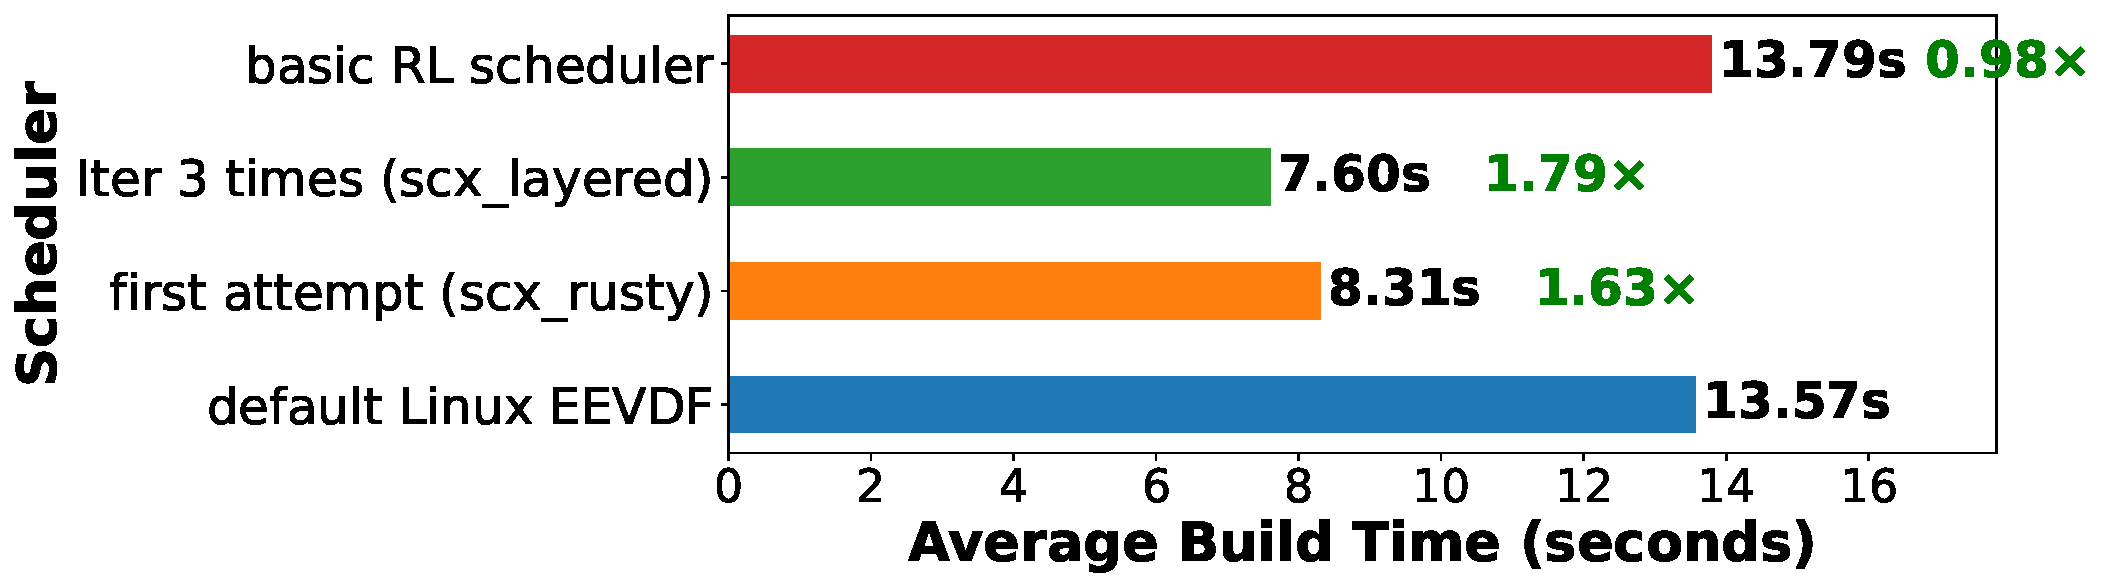
\includegraphics[width=0.9\columnwidth]{sections/Linux_build_benchmark_results.pdf}
\caption{Performance comparison of scheduler configurations in Linux build benchmark.}
\label{fig:performance-comparison}
\end{figure}

We further evaluate \sys on machine 2 using schbench~\cite{schbench2016}, a scheduler benchmark measuring wakeup latency and throughput. Figure~\ref{fig:schbench-comparison} compares three configurations: default EEVDF, initial selection (scx\_bpfland), and iterative optimization (scx\_rusty after 3 iterations). While AI configured scheduler initially underperformed with 13\% worse P99 latency (46.1ms vs 40.3ms) and 19\% lower throughput (741 vs 910 req/s), AI iterative refinement identified scx\_rusty as superior. After three iterations, scx\_rusty achieved 2.11× better P99 latency (19.1ms) and 1.60× higher throughput (1452 req/s) versus EEVDF, demonstrating our agent's effective learning from performance feedback.

\begin{figure}[h]
\centering
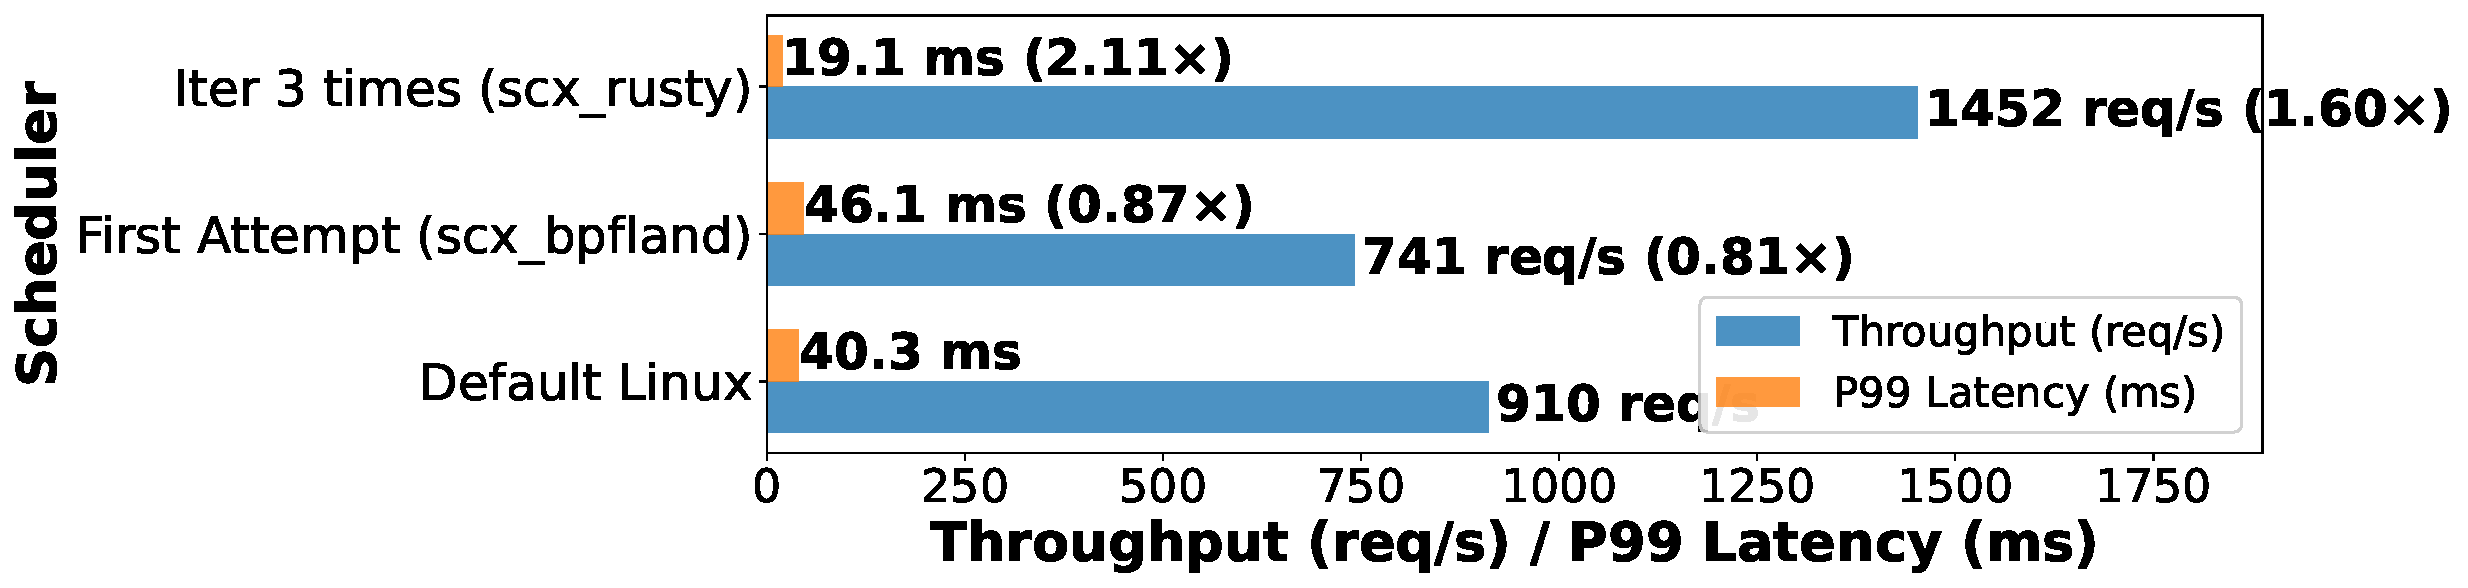
\includegraphics[width=0.9\columnwidth]{sections/schbench_performance_comparison.pdf}
\caption{Schbench performance comparison showing P99 latency and throughput improvements through iterative scheduler optimization.}
\label{fig:schbench-comparison}
\end{figure}

\subsection{AI-Generated Schedulers for Batch Workloads}

Figure~\ref{fig:batch-performance} evaluates the \sys  and \agent  ability to generate new schedulers from scratch (not merely select existing ones) on 8 diverse batch workloads (e.g. file compression, video transcoding, software testing, and data analytics tasks) running on machine 2. To simulate a long-tail distribution, each workload comprised 40 parallel tasks: 39 short and one significantly longer, each as a python script or C/C++ program. The agent consistently identified this pattern and generated custom eBPF code implementing a Longest Job First (LJF) scheduling policy—a scheduler not present in our repository—achieving an average 20\% reduction in end-to-end processing time. The cost for this analysis averaged \$0.15 per workload, based on Claude Opus 4 pricing from August 2025. We note that the powerful Claude Opus agent successfully classified all 8 workloads, whereas the smaller Claude Sonnet model could not. In addition to performance gains, our framework's optimizations reduced generation costs per iteration: time fell from 33 to 2.5 minutes (a 13x reduction), and the monetary cost dropped from \$6 to \$0.5.

\begin{figure}[h]
\centering
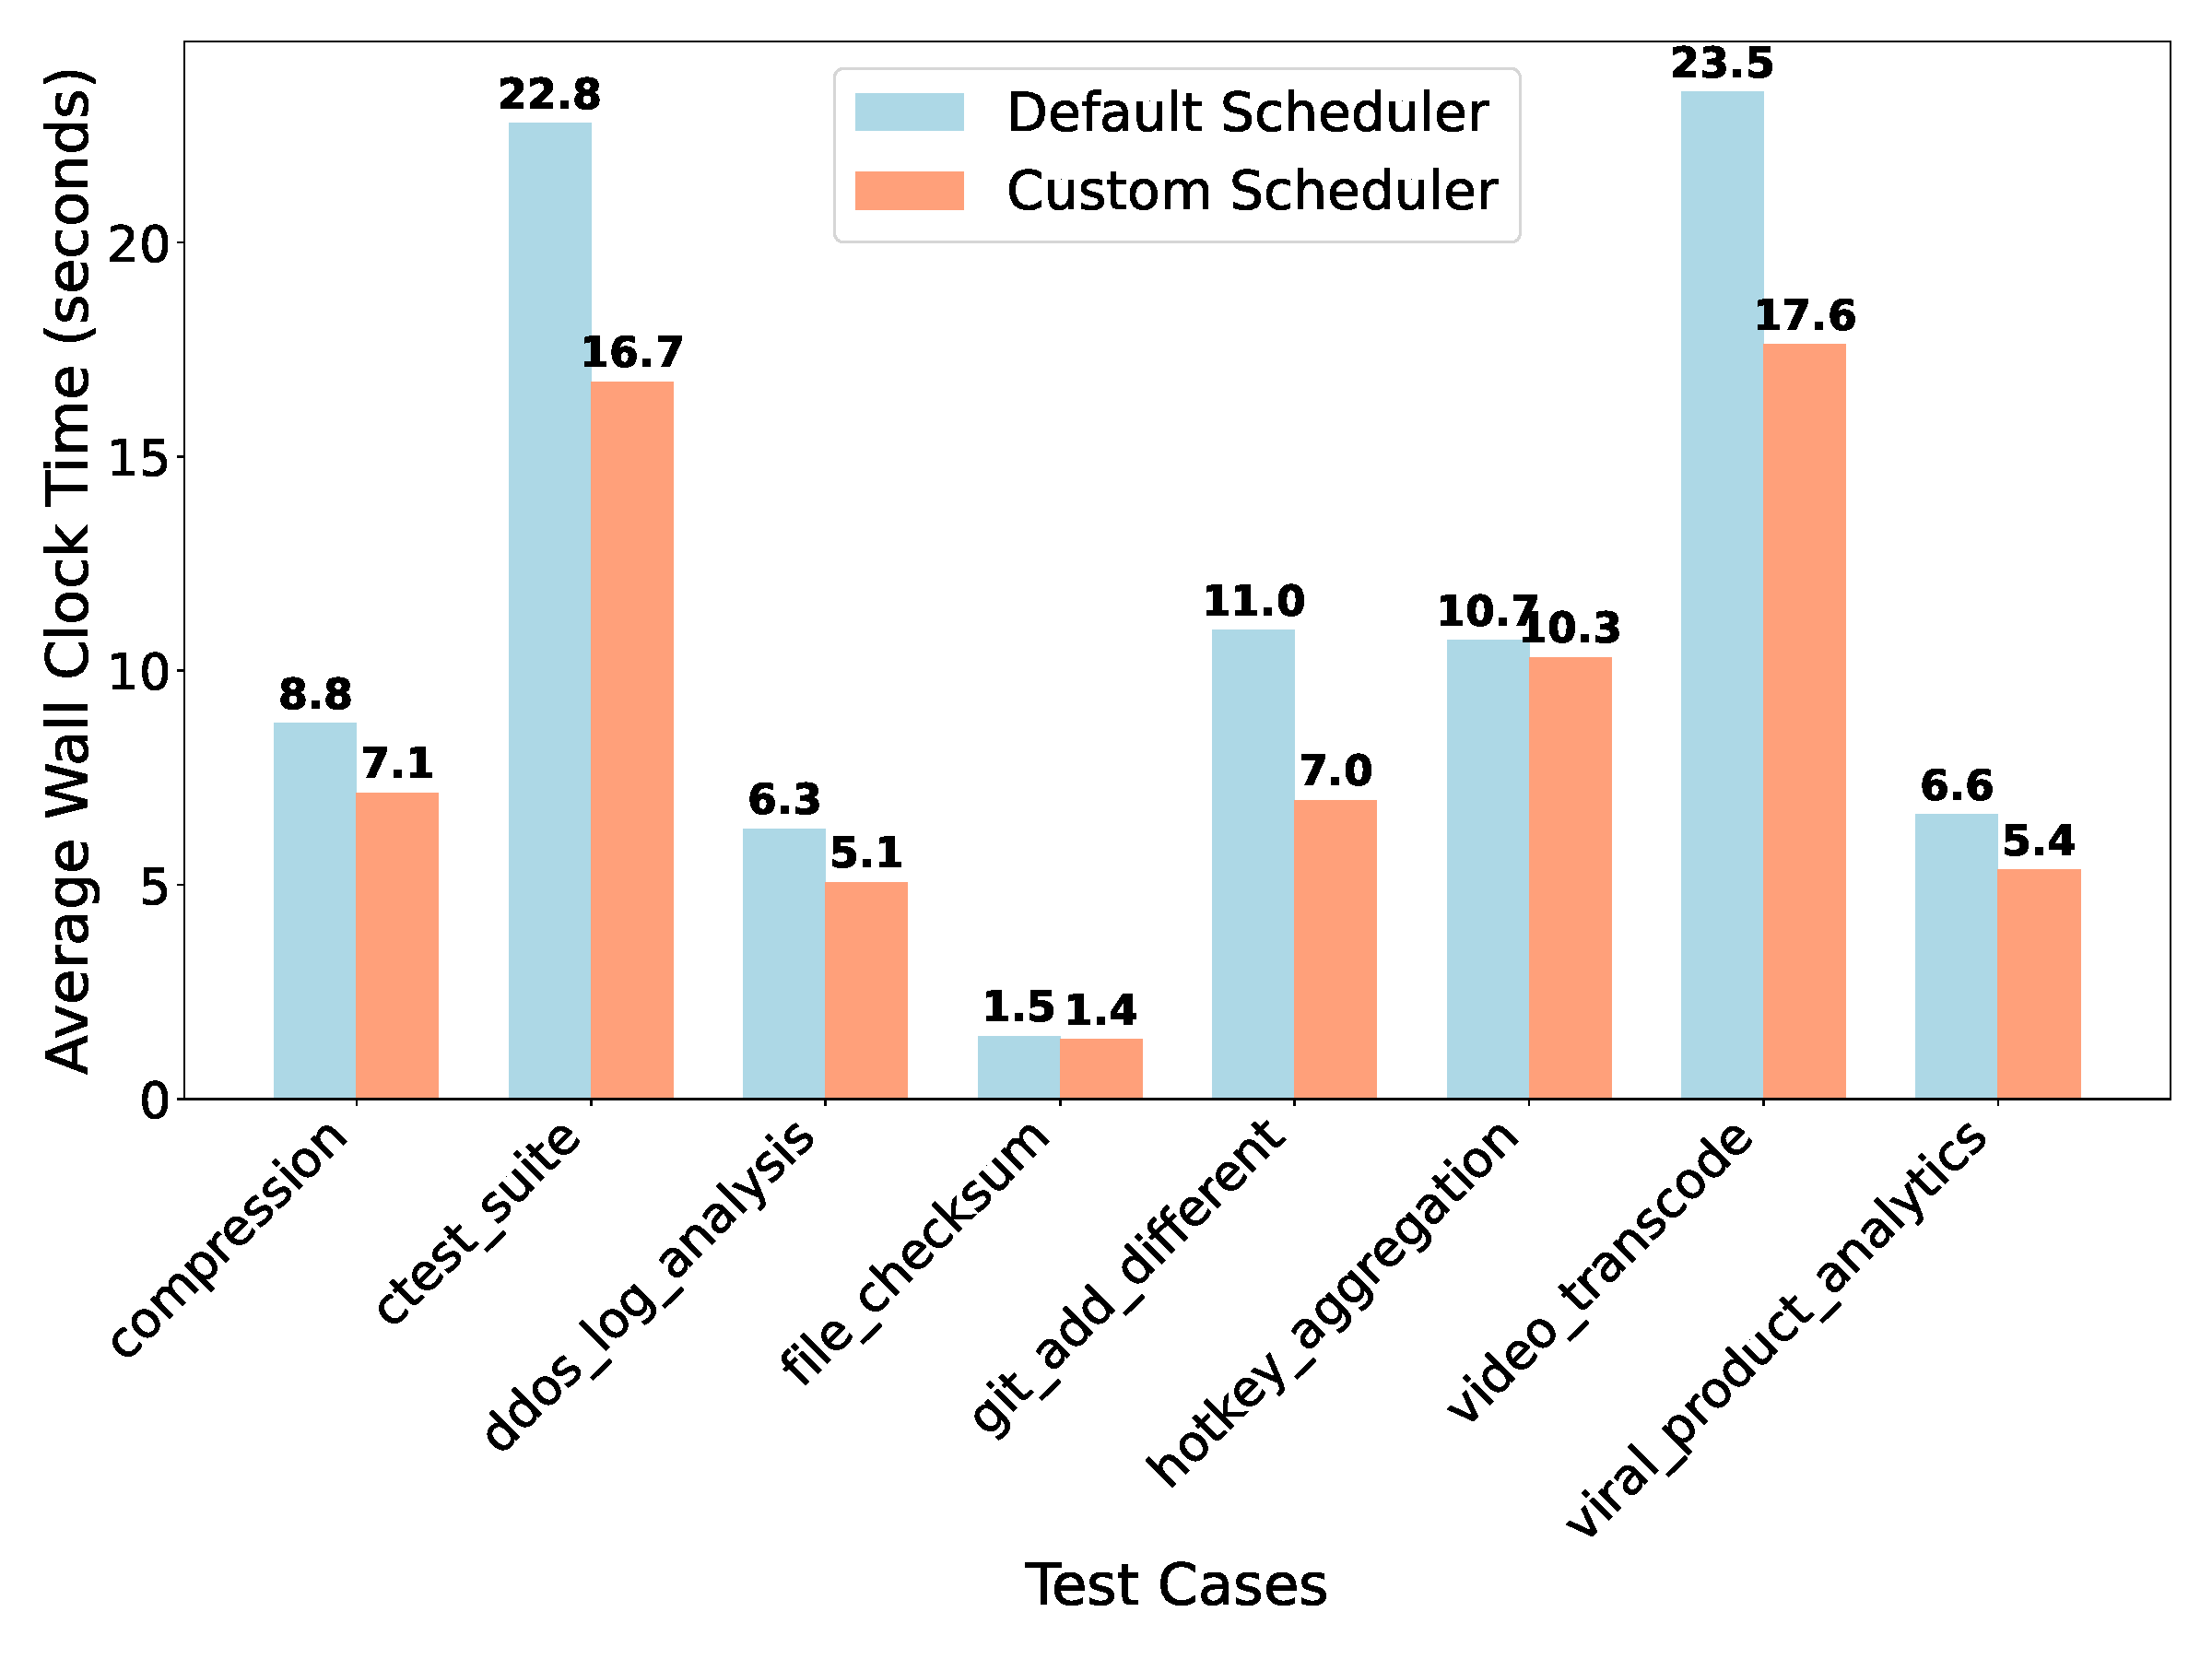
\includegraphics[width=0.9\columnwidth]{sections/scheduler_performance_comparison.pdf}
\caption{AI-generated scheduler performance on batch workloads.}
\label{fig:batch-performance}
\end{figure}


